% vim: set tw=78 sts=2 sw=2 ts=8 aw et ai:

Proper implementation is proper.

Another module of our project is represented by the Encoding module. As we
have previously mentioned, the TCP header options field offers us 37 useful
bytes. Although this is a greater capacity than other protocols offer, it is
still a limited amount, so we have to use it properly.

The first thing to do is minimize the size of the input data (the useful
data encapsulated inside the TCP header), which leads to the idea of compressing
it. Our communication must be reliable and entirely exact, pointing to an
approach based on a lossless data compression algorithm. One of the most
suitable lossless algorithms is Huffman coding.

Huffman coding\cite{huffman1952method} is an entropy encoding algorithm using
a variable-length code table for encoding source symbols (characters in the
current situation), where the table is generated based on the probabilities of
occurence for each of the source symbols. In the end, what you get is a binary
tree of nodes which provides you unique combinations of bits for all the
symbols.

Practically speaking, the compression technique works in the following way:
first, all the nodes are leaf nodes, which contain the symbol itself and the
frequency of occurence; then the nodes are taken two by two starting with the
smallest frequencies, joining them by a common parent containing the sum of
their frequencies; the process is repeated until you have a single root node;
the edges are given bit values (0 the left branches, 1 the right branches);
the encoding for each letter is calculated by following the path of bits from
the root to the corresponding leaf.

\begin{figure}
  \centering
  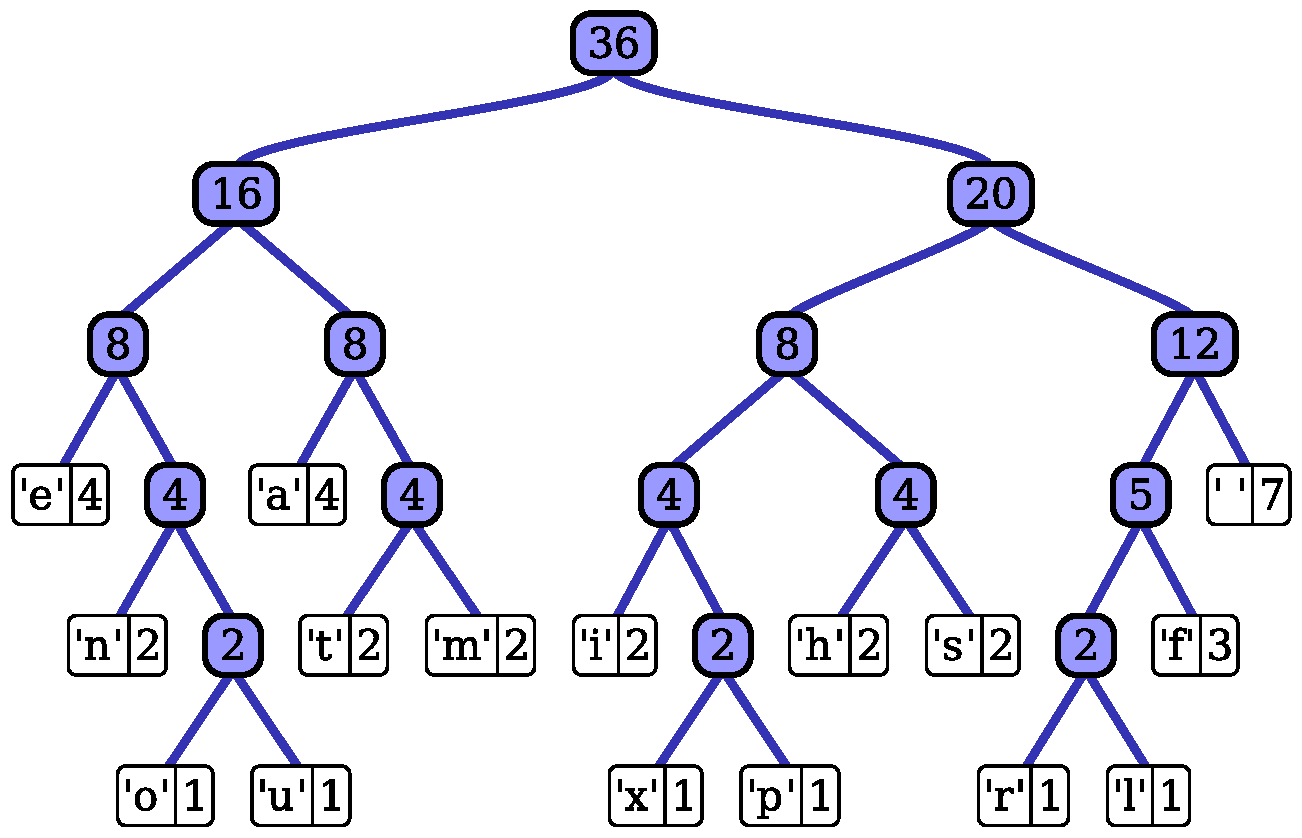
\includegraphics[width=0.5\textwidth]{img/huffman}
  \caption{Huffman tree generated for "this is an example of a huffman tree"}
  \label{fig:huffman}
\end{figure}

Reffering to the example in Figure \ref{fig:huffman}, the code for 'e' would
be '000', for 'a' '010', for 'u' '00111', and so on. As you can see, the most
frequent characters have the shortest codes.

In order to create a working encoding module, we have implemented the Huffman
algorithm to encode / compress the payload of our message. The result is a
sequence of bits to be added in the 37 bytes left of the options field.

But the things weren't that simple. First of all, the message had to be decoded
when it arrived at the destination. For this to be accomplished, we needed to
send the codebook along with the encoded message, so the first bytes of the
field had to define the length of the codebook and describe the codebook itself.

Another problem to overcome was to be continued...








